\documentclass[border=0pt]{standalone}
\usepackage{fontspec}
\setmainfont{Geist-Regular.ttf}[Path=./]
\newfontfamily\mono{GeistMono-Regular.ttf}[Path=./]
\usepackage{xcolor}
\usepackage{tikz}
\usetikzlibrary{arrows.meta,calc,fit,backgrounds}

\definecolor{ink}{HTML}{141413}
\definecolor{paper}{HTML}{FBFAF7}
\definecolor{muted}{HTML}{6B6A66}
\definecolor{cClient}{HTML}{EDEBE6}
\definecolor{cFront}{HTML}{DCE6F2}
\definecolor{cPush}{HTML}{F6DFCC}
\definecolor{cFetch}{HTML}{D7EBDD}
\definecolor{cStore}{HTML}{E6DEF0}
\definecolor{cMeta}{HTML}{F3E7B8}
\definecolor{cComp}{HTML}{EFE2DA}
\definecolor{cLoop}{HTML}{F6F4EC}
\definecolor{accent}{HTML}{C8423B}

\newcommand\ti[1]{{\fontsize{15}{17}\selectfont #1}}
\newcommand\su[1]{{\fontsize{10.5}{13}\selectfont\color{muted}#1}}

\tikzset{
  box/.style={draw=ink, line width=1pt, rounded corners=5pt, align=center,
              minimum width=4.6cm, minimum height=2.1cm, inner sep=6pt, text=ink},
  arr/.style={-{Stealth[length=7pt,width=6pt]}, line width=0.9pt, draw=ink},
  dashedarr/.style={arr, dash pattern=on 5pt off 3pt},
  lab/.style={fill=paper, inner sep=2.5pt, align=center, font=\fontsize{10.5}{12.5}\selectfont, text=ink},
  mlab/.style={lab, font=\mono\fontsize{9.5}{11.5}\selectfont},
}

\begin{document}
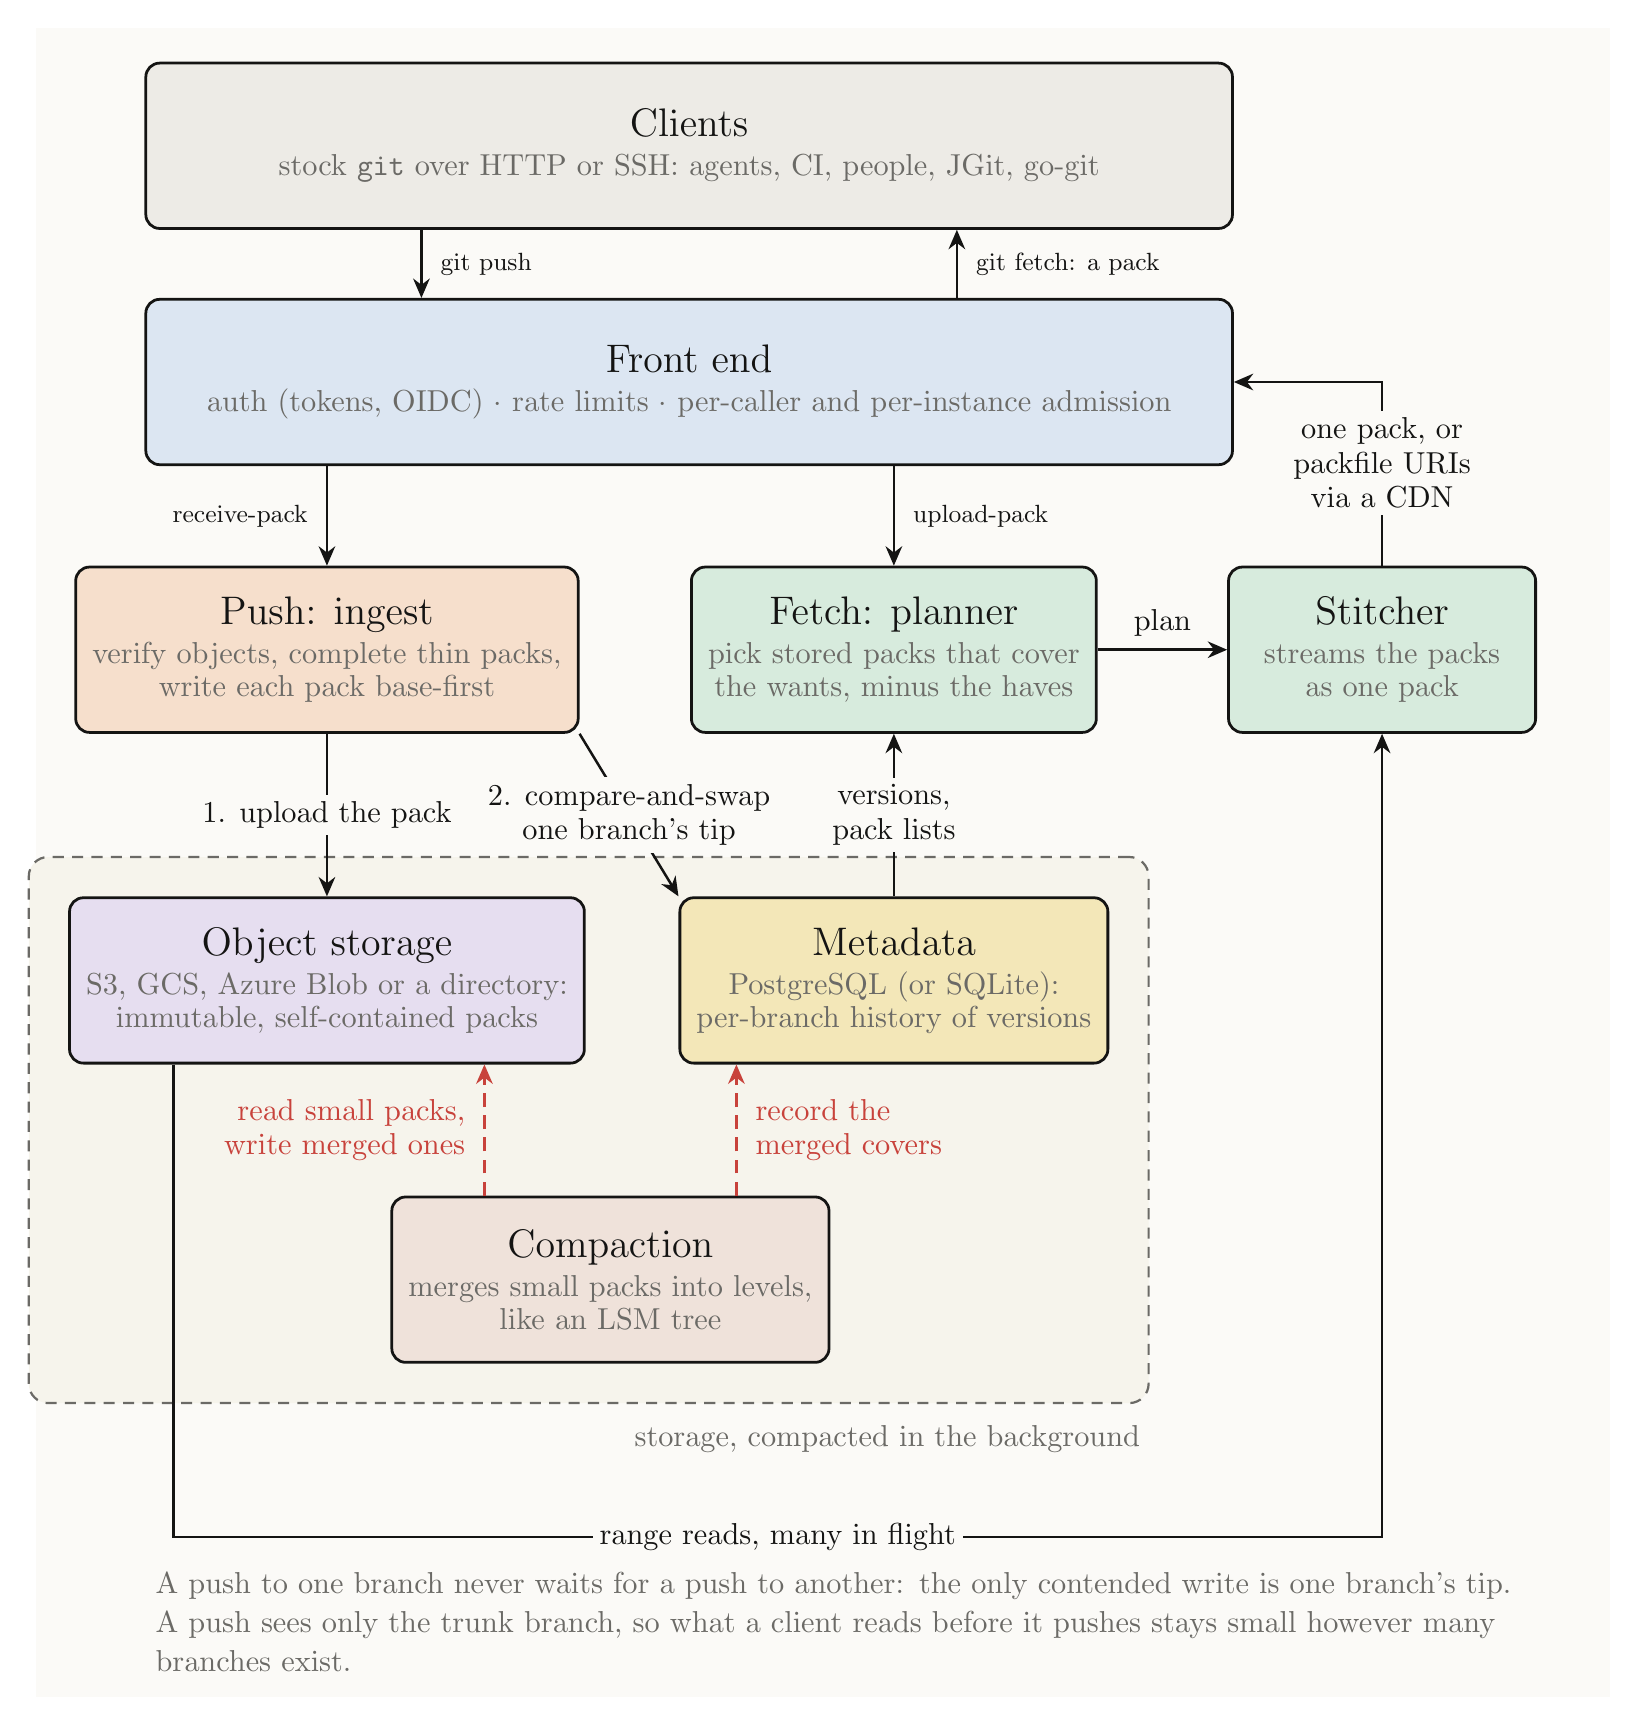
\begin{tikzpicture}
  \begin{scope}[on background layer]\fill[paper] (-3.7,3.9) rectangle (16.3,-17.3);\end{scope}
  \node[box, fill=cClient, minimum width=13.8cm] (clients) at (4.6,2.4)
    {\ti{Clients}\\[2pt]\su{stock \texttt{git} over HTTP or SSH: agents, CI, people, JGit, go-git}};
  \node[box, fill=cFront, minimum width=13.8cm] (front) at (4.6,-0.6)
    {\ti{Front end}\\[2pt]\su{auth (tokens, OIDC) \(\cdot\) rate limits \(\cdot\) per-caller and per-instance admission}};

  \node[box, fill=cPush] (ingest) at (0,-4.0)
    {\ti{Push: ingest}\\[2pt]\su{verify objects, complete thin packs,}\\\su{write each pack base-first}};
  \node[box, fill=cFetch] (plan) at (7.2,-4.0)
    {\ti{Fetch: planner}\\[2pt]\su{pick stored packs that cover}\\\su{the wants, minus the haves}};
  \node[box, fill=cFetch, minimum width=3.9cm] (stitch) at (13.4,-4.0)
    {\ti{Stitcher}\\[2pt]\su{streams the packs}\\\su{as one pack}};

  \node[box, fill=cStore] (s3) at (0,-8.2)
    {\ti{Object storage}\\[2pt]\su{S3, GCS, Azure Blob or a directory:}\\\su{immutable, self-contained packs}};
  \node[box, fill=cMeta] (pg) at (7.2,-8.2)
    {\ti{Metadata}\\[2pt]\su{PostgreSQL (or SQLite):}\\\su{per-branch history of versions}};
  \node[box, fill=cComp] (compact) at (3.6,-12.0)
    {\ti{Compaction}\\[2pt]\su{merges small packs into levels,}\\\su{like an LSM tree}};

  \begin{scope}[on background layer]
    \node[draw=muted, line width=0.8pt, dash pattern=on 4pt off 3pt, rounded corners=7pt, fill=cLoop,
          fit=(s3)(pg)(compact), inner sep=0.5cm] (loopbox) {};
  \end{scope}
  \node[anchor=north east, font=\fontsize{11}{13}\selectfont\color{muted}] at ([yshift=-4pt]loopbox.south east)
    {storage, compacted in the background};

  % clients <-> front
  \draw[arr] ([xshift=-3.4cm]clients.south) -- node[mlab,right=4pt,fill=none]{git push} ([xshift=-3.4cm]front.north);
  \draw[arr] ([xshift=3.4cm]front.north) -- node[mlab,right=4pt,fill=none]{git fetch: a pack} ([xshift=3.4cm]clients.south);

  % front -> paths
  \draw[arr] (front.south -| ingest.north) -- node[mlab,left=4pt,fill=none]{receive-pack} (ingest.north);
  \draw[arr] (front.south -| plan.north) -- node[mlab,right=4pt,fill=none]{upload-pack} (plan.north);

  % push path
  \draw[arr] (ingest.south) -- node[lab]{1. upload the pack} (s3.north);
  \draw[arr] (ingest.south east) -- node[lab]{2. compare-and-swap\\one branch's tip} (pg.north west);

  % fetch path
  \draw[arr] (pg.north) -- node[lab]{versions,\\pack lists} (plan.south);
  \draw[arr] (plan.east) -- node[lab,above=2pt,fill=none]{plan} (stitch.west);
  \draw[arr] ([xshift=-1.95cm]s3.south) -- ++(0,-6.0) -| node[lab,pos=0.25]{range reads, many in flight} (stitch.south);
  \draw[arr] (stitch.north) |- node[lab,pos=0.28]{one pack, or\\packfile URIs\\via a CDN} (front.east);

  % compaction
  \draw[dashedarr, draw=accent] ([xshift=-1.6cm]compact.north) -- node[lab,left=4pt,text=accent,fill=none,align=right]{read small packs,\\write merged ones} ([xshift=-1.6cm]compact.north |- s3.south);
  \draw[dashedarr, draw=accent] ([xshift=1.6cm]compact.north) -- node[lab,right=4pt,text=accent,fill=none,align=left]{record the\\merged covers} ([xshift=1.6cm]compact.north |- pg.south);

  \node[anchor=north west, align=left, text width=17.6cm, font=\fontsize{10.5}{14}\selectfont, text=muted]
    at (-2.3,-15.6)
    {A push to one branch never waits for a push to another: the only contended write is one branch's tip.
     A push sees only the trunk branch, so what a client reads before it pushes stays small however many branches exist.};

\end{tikzpicture}
\end{document}
